\documentclass[12pt,ngerman]{scrartcl}

\usepackage[autoprint]{pythontex}
\usepackage{booktabs}
\usepackage{amsmath}
\usepackage{graphicx}
\begin{document}

Hallo

\py{1+1}

\[
2^{100}=\py{2**100}
\]


\begin{pycode}
from sympy import *
x, y = symbols("x y")
binome = []
for exponent in range(3, 7):
    binome.append((x + y)**exponent)
    print(r"\begin{align*}")
    for expr in binome:
        print(r"%s &= %s\\" % (latex(expr), latex(expand(expr))))
    print(r"\end{align*}")
\end{pycode}

\begin{pycode}
from pylab import *
def f(t):
    return cos(3 * pi * t) * exp(-t)

t = linspace(0, 10, 500)
y = f(t)
clf()
figure(figsize=(5, 3))
rc("text", usetex=True)
plot(t, y)
title(r'Ged\"ampfter exponentieller Zerfall') 
text(6, 0.15, r"$y = \cos(2 \pi t) e^{-t}$")
xlabel("Zeit (t)")
ylabel("Spannung (mV)")
savefig("zerfall.pdf", bbox_inches="tight")
print(r"\begin{center}")
print(r"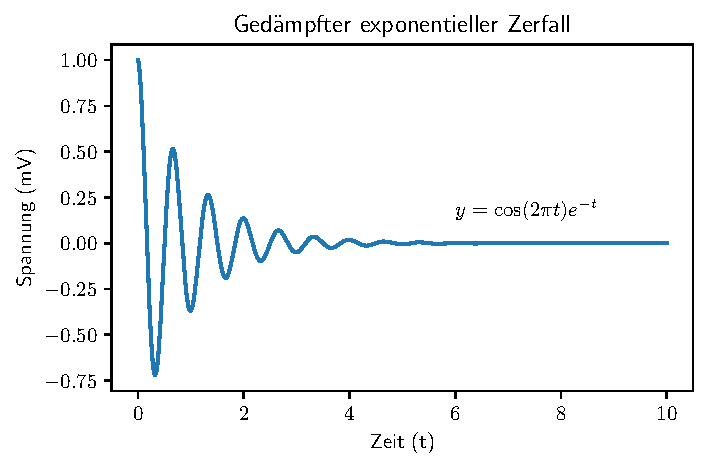
\includegraphics[width=0.6\textwidth]{zerfall.pdf}")
print(r"\end{center}")
\end{pycode}


\end{document}